\documentclass{article}
\usepackage{physics}
\usepackage{graphicx}
\usepackage{caption}
\usepackage{amsmath}
\usepackage{authblk}
\usepackage{amsfonts}
\usepackage{esint}
\usepackage{mathtools}
\usepackage{amsthm}
\theoremstyle{definition}
\newtheorem{defn}{Definition}[section]
\newtheorem{prop}{Proposition}[section]
\newtheorem{rmk}{Remark}[section]
\newtheorem{exmp}{Example}[section]
\usepackage{empheq}
\usepackage{hyperref}
\usepackage{tensor}
\usepackage{xcolor}
\hypersetup{
	colorlinks,
	linkcolor={black!50!black},
	citecolor={blue!50!black},
	urlcolor={blue!80!black}
}
\usepackage[english]{babel}
\usepackage[utf8]{inputenc}
\usepackage{fancyhdr}

\pagestyle{fancy}
\fancyhf{}
\rhead{Huan Q. Bui}
\lhead{Electromagnetically Induced Transparency}
\rfoot{\thepage}

\begin{document}
\section{Introduction}
The following introduction to Electromagnetically Induced Transparency (EIT) is based on Stephen E. Harris' article in \textit{PHYSICS TODAY}, 1997. \href{https://web.stanford.edu/group/harrisgroup/PAPERS/review.pdf}{\underline{Link}}, and various other sources including this well-written \href{https://www.reed.edu/physics/faculty/illing/campus/pdf/FurmanThesis16.pdf}{\underline{thesis}} by Furman of Reed College, this \href{https://www.kip.uni-heidelberg.de/kw/image/f/group/f17/files/F65_EIT_Anleitung.pdf}{paper}, and of course \textit{Principles of Laser Spectroscopy and Quantum Optics} by Paul Berman.\\

In shortest possible terms, EIT is a technique which renders an otherwise opaque atomic medium transparent with electromagnetic radiation. The medium is typically a \href{http://community.dur.ac.uk/thomas.billam/JQC_Atom_Light_2015-2016_L7.pdf}{\underline{three-level}} atomic system, with specific requirements: two of the possible three transitions must be dipole-allowed (so transition rules satisfied) and one not dipole-allowed. The spectrum of the medium without (blue) and with (red) EIT is shown below:
\begin{figure}[h!]
\centering
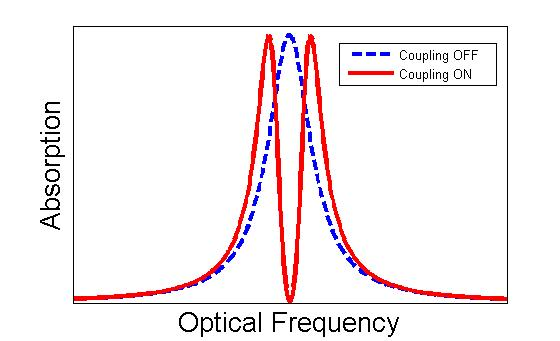
\includegraphics[scale=0.5]{EIT_spectrum.jpg}
\caption{}
\end{figure}

Notice how there is no absorption at resonance frequency with EIT. Typically, in the presence of a near-resonance field, a two-level atom with ground state $\ket{1}$ and excited state $\ket{2}$ will interact with the field, resulting in a non-zero probability amplitude of the excited state, $\vert P_2\vert^2 = \bra{2}\ket{2} > 0$. If $\vert P_2(\delta\omega) \vert^2$ is the population of the excited state as a function of the detuning, then it follows the blue, Lorentzian line in the above figure. In EIT where there are two radiation fields, though, the energy levels of a three-level atom are altered. This in turn creates a window of frequencies at which the medium is transparent. \\

\section{Derivation Overview}

The following derivation is (heavily) inspired by Furman's derivation and the Heidelberg paper, but roughly condensed and sprinkled with a bit of my own narratives and insights here and there. \\

Let's consider a $\Lambda$ configuration:
\begin{figure}[h!]
	\centering
	\includegraphics[scale=0.5]{Lambda.PNG}
	\caption{}
\end{figure}

Let the energy of each state $\ket{n}$, $n=\{1,2,3\}$ be
\begin{align}
E_n = \bra{i}\hat{H}\ket{n} = \hbar\omega_n.
\end{align}
where $\hat{H}$ is the neutral atom Hamiltonian. Assume that the transition $\ket{1} \rightarrow \ket{2}$ is forbidden (just as shown in Figure 2). Since $E_n$ and $\ket{n}$ are the eigenvalues and eigenstates of $\hat{H}$, respectively, we let the bare-atom Hamiltonian $\hat{H_0}$ be:
\begin{align}
\hat{H_0}=
\hbar\begin{pmatrix}
\omega_1 & 0 & 0\\
0 & \omega_2 & 0\\
0 & 0 & \omega_3
\end{pmatrix}.
\end{align}
We can do this because the eigenstates $\ket{n}$ form an orthonormal basis. Next, let the applied fields be 
\begin{align}
\vec{E} &= \vec{E}_p \cos(\omega_p t - \vec{k_p}\cdot\vec{r}) +
\vec{E}_c \cos(\omega_c t - \vec{k_c}\cdot\vec{r}) \nonumber\\
&\approx \vec{E}_p \cos(\omega_p t) +
\vec{E}_c \cos(\omega_c t)\nonumber\\
&= \frac{\vec{E}_p}{2}\left(e^{i\omega_pt} - e^{-i\omega_pt} \right) + \frac{\vec{E}_c}{2}\left( e^{i\omega_ct} + e^{i\omega_ct}\right). 
\end{align}
where $\omega_p \approx \omega_{13} = \omega_3 - \omega_1$, and $\omega_c \approx \omega_{23} = \omega_3 - \omega_2$. The subscripts $p$ and $c$ means \textbf{probe} and \textbf{coupling}, respectively. We should also denote the relevant detuning $\delta_p = \omega_{13} - \omega_p$ and $\delta_c = \omega_{12} - \omega_c$. It makes sense to label our subscripts this way, because in the end we are interested in the probability amplitude of $\ket{3}$ as a function of the detuning $\delta_p$ of the probe beam from (bare atom) resonance.\\

With the perturbation from the radiation, the new Hamiltonian of the atom is:
\begin{align}
\hat{H} = \hat{H}_0 + \hat{H}_1,
\end{align}
where, with $\hat{\rho} \equiv qd$ being the dipole moment operator:
\begin{align}
\hat{H}_{1,ij} = -E\hat{\rho}_{ij},
\end{align}
where $E$ is the field strength. We will see how $E$ relates to the Rabi rate $\Omega$ later. Now, a state does not dipole-interact with itself, hence $\rho_{ii} = 0$. In addition, since the transition $\ket{1} \rightarrow \ket{2}$ is forbidden, $\rho_{12} = \rho{21} = 0$. It follows that:
\begin{align}
\hat{H} &= \hat{H}_0 + \hat{H}_1 \nonumber\\
&= \hbar\begin{pmatrix}
\omega_1 & 0 & 0\\
0 & \omega_2 & 0\\
0 & 0 & \omega_3
\end{pmatrix} -
E\begin{pmatrix}
0 & 0 & \rho_{13}\\
0 & 0 & \rho{23}\\
\rho_{31} & \rho_{32} & 0
\end{pmatrix}.
\end{align}
Now, what we have been working with so far are the time-independent eigenstates $\ket{n}$. In the following steps we shall bring in the time-dependent parts. To do this, we invoke the unitary matrix $U(t)$, which transforms $\ket{n}$ into full time-dependent wavefunctions:
\begin{align}
U(t) = e^{iH_0t/\hbar}
\begin{pmatrix}
e^{i\omega_1t} & 0 & 0\\
0 & e^{i\omega_2t} & 0\\
0 & 0 & e^{i\omega_3t}
\end{pmatrix}.
\end{align} 
Obviously, if we apply $\hat{U}(t)$ to $\hat{H}_0$ there wouldn't be anything interesting, since $\hat{U}(t) = d/dt\hat{H}_0$. But we can apply $\hat{U}(t)$ to $\hat{H}_1$. The change of basis rule gives
\begin{align}
\hat{U}(t)\hat{H}_1\hat{U}^{\dagger}(t) = 
-E\begin{pmatrix}
0 & 0 & \rho_{13}e^{-i\omega_{13}t}\\
0 & 0 & \rho_{23}e^{-i\omega_{23}t}\\
\rho_{31}e^{i\omega_{13}t} & \rho_{32}e^{i\omega_{32}t} & 0
\end{pmatrix}.
\end{align}
Multiplying $E$ into $\hat{H}_1$ and applying rotating wave approximation to result gives the non-zero matrix elements:
\begin{align}
\left( \hat{U}(t)\hat{H}_1\hat{U}^\dagger\right)_{13} &= 
-\frac{1}{2}E_p \rho_{13}e^{i(\omega_p - \omega_{13})t}\\
\left( \hat{U}(t)\hat{H}_1\hat{U}^\dagger\right)_{23} &= 
-\frac{1}{2}E_c \rho_{23}e^{i(\omega_c - \omega_{23})t}\\
\left( \hat{U}(t)\hat{H}_1\hat{U}^\dagger\right)_{31} &= 
-\frac{1}{2}E_p \rho_{31}e^{i(\omega_p - \omega_{31})t}\\
\left( \hat{U}(t)\hat{H}_1\hat{U}^\dagger\right)_{32} &= 
-\frac{1}{2}E_c \rho_{32}e^{i(\omega_c - \omega_{32})t}
\end{align}
Transforming $\hat{H}_1$ back to the vector space of $\ket{n}$ gives:
\begin{align}
\hat{H_1} &= \hat{U}^\dagger(t) \left( \hat{U}(t) \hat{H}_1 \hat{U}^\dagger(t)\right) \hat{U}(t) \nonumber \\
&= 
-\frac{1}{2}\begin{pmatrix}
0 & 0 & E_p\rho_{13}e^{i\omega_pt}\\
0 & 0 & E_c\rho_{23}e^{i\omega_ct}\\
E_p\rho_{31}e^{-i\omega_pt} & E_c\rho_{32}e^{-i\omega_ct} & 0
\end{pmatrix}.
\end{align}
Now, to put the dipole moment in terms of the Rabi frequency $\Omega$:
\begin{align}
\Omega_p = \frac{E_p\vert \rho_{13} \vert}{\hbar} &= \frac{E_p\rho_{13}e^{-i\phi_p}}{\hbar}\\
\Omega_c = \frac{E_c\vert \rho_{23} \vert}{\hbar} &= \frac{E_c\rho_{23}e^{-i\phi_c}}{\hbar}
\end{align}
So the total Hamiltonian is
\begin{align}
\hat{H} = \frac{\hbar}{2}
\begin{pmatrix}
2\omega_1 & 0 & -\Omega_pe^{i(\omega_pt+\phi_p)}\\
0 & 2\omega_2 & -\Omega_ce^{i(\omega_ct+\phi_c)}\\
-\Omega_pe^{-i(\omega_pt+\phi_p)} & -\Omega_ce^{-i(\omega_ct+\phi_c)} & 2\omega_3
\end{pmatrix}
\end{align}
Now, since we want our final result in terms of the frequencies only, we shall express $\hat{H}$ in a new basis that is time and phase independent. Let a unitary matrix $\tilde{U}(t)$ be given such that it satisfies the required change of basis. It follows that the eigenstates transform as
\begin{align}
\ket{\tilde{n}} = \tilde{U}(t)\ket{n'}.
\end{align}
Let the new Hamiltonian in this new basis be $\tilde{H}$. The new eigenstate also has to solve the Schr\"{o}dinger equation in the new basis, so
\begin{align}
\tilde{H}\ket{\tilde{n}} &= i\hbar \frac{\partial }{\partial t}\ket{\tilde{n}}\nonumber \\
&= i\hbar\frac{\partial}{\partial t}\left(\tilde{U}\ket{n'} \right) \nonumber\\
&= i\hbar\left( \frac{\partial \tilde{U}}{\partial t}\ket{n'} + \tilde{U}\frac{\partial}{\partial t}\ket{n'}\right)\nonumber\\
&=  i\hbar\left( \frac{\partial \tilde{U}}{\partial t}\ket{n'} + \frac{1}{i\hbar}\tilde{U}\hat{H}\ket{n'}\right) \nonumber\\
&= \left(i\hbar \frac{\partial \tilde{U}}{\partial t}\tilde{U}^\dagger + \tilde{U}\hat{H}\tilde{U}^\dagger \right) \tilde{U}\ket{n'}\nonumber\\
&= \left(i\hbar \frac{\partial \tilde{U}}{\partial t}\tilde{U}^\dagger + \tilde{U}\hat{H}\tilde{U}^\dagger \right) \ket{\tilde{n}}.
\end{align}
So $\tilde{H}$ can be readily computed:
\begin{align}
\tilde{H} &= \left(i\hbar \frac{\partial \tilde{U}}{\partial t}\tilde{U}^\dagger + \tilde{U}\hat{H}\tilde{U}^\dagger \right)\nonumber\\
&= \frac{\hbar}{2}\begin{pmatrix}
2(\omega_1 + \omega_p) & 0 & \Omega_p\\
0 & 2(\omega_2+\omega_c) & -\Omega_c\\
-\Omega_p & -\Omega_c & 2\omega_3
\end{pmatrix}
\end{align}
Note that we can add $\hbar(\omega_1+\omega_p)\hat{I}$ to $\tilde{H}$ without changing the physical interpretation. In fact, the form of $\tilde{H}$ now is a result of our definition of the $\omega$'s. Now, let us define the detunings $\delta_c = \omega_{23}-\omega_c = \omega_3 - \omega_2 - \omega_c $ and $\delta_p = \omega_{13} - \omega_p = \omega_3 - \omega_1 - \omega_p$. So, the ``better'' Hamiltonian is
\begin{align}
\tilde{H}' &= \tilde{H} - \hbar(\omega_1+\omega_p)\hat{I}\nonumber\\
&= \hbar\begin{pmatrix}
0 & 0 & -\Omega_p\\
0 & 2(\delta_p - \delta_c) & -\Omega_c\\
-\Omega_p & -\Omega_c & 2\delta_p
\end{pmatrix}
\end{align}
The eigenvalues of $\tilde{H}'$ are:
\begin{align}
&E^+ = \hbar\omega^+ = \frac{\hbar}{2}\left( \delta_p + \sqrt{\delta^2_p + \Omega^2_p + \Omega^2_c}\right) \nonumber\\
&E^- = \hbar\omega^- = \frac{\hbar}{2}\left( \delta_p - \sqrt{\delta^2_p + \Omega^2_p + \Omega^2_c}\right) \nonumber\\
&E^0 = \hbar\omega = 0.
\end{align}
And the eigenstates are:
\begin{align}

\end{align}











	
\end{document}